\documentclass[UTF8,a4paper]{ctexart}
\usepackage[utf8]{inputenc}
\usepackage{amsmath}
\usepackage{pdfpages}
\usepackage{graphicx}
\usepackage{wrapfig}
\usepackage{listings}
\usepackage{xcolor}
\lstset{
    numbers=left, 
    numberstyle= \tiny, 
    keywordstyle= \color{ blue!70},
    commentstyle= \color{red!50!green!50!blue!50}, 
    frame=shadowbox, % 阴影效果
    rulesepcolor= \color{ red!20!green!20!blue!20} ,
    escapeinside=``, % 英文分号中可写入中文
    xleftmargin=2em,xrightmargin=2em, aboveskip=1em,
    framexleftmargin=2em
} 
\title{计算机原理第一次实验报告}
\author{张蔚桐\ 2015011493\ 自55}
\begin {document}
\maketitle
\section{实验内容}
\subsection{DEBUG的使用练习}
启动DEBUG, 用A 命令输入实验指导书中程序段,用U 命令对此程序作反汇编,在显示屏上逐行阅读程序,并将机器语言和助记符对照,体会机器码和指令助记符(尤其是指令中的立即数) 之间的对应关系。分别用G、P 及T命令执行此程序,并随时用D 及R 命令检查有关内存单元及寄存器内容。本程序在一块数据区写入了0~F 十六个数,用D 命令可以看到相应数据区内容在程序运行前后的变化,用W 命令将程序存于磁盘,用L 命令将程序取回并反汇编检查程序是否复原。
\subsection{汇编语言上机}
用文本编辑器完成以下汇编程序,保存后采用TASM和LINK先后进行编译和连接。在debug模式下检查程序执行和内存变化情况,发现程序完成了内存段的拷贝和语句输出
\lstinputlisting{p12.asm}
\subsection{选做内容}
在上面汇编代码的基础上进行修改,利用循环和累加的操作完成对30H~39H 及41H~46H的写入操作
\lstinputlisting{p13.asm}
\section{程序运行情况}
1.1中的程序0H~FH 依次存放在DS:0200~DS:020F 中。首先将SI、CX、AL 初始化,每次将AL 中的值传到DS:[SI] 指向的内存中,地址SI、内容AL 加1,CX 计数减1。循环10 次后,通过INT 结束程序。

1.2中的程序通过累加和循环完成内存块之间的拷贝工作

1.3中的选做程序通过累加和两段循环的方式完成对内存块的写入工作,和1.2不同的是,采用了LOOP命令进行流程控制
\section{总结}
通过这次实验,我熟悉了DOS环境和DEBUG的相关使用方法,对汇编语言也有了更多的体验和了解。为后续实验做好了准备
\begin{figure}
\centering
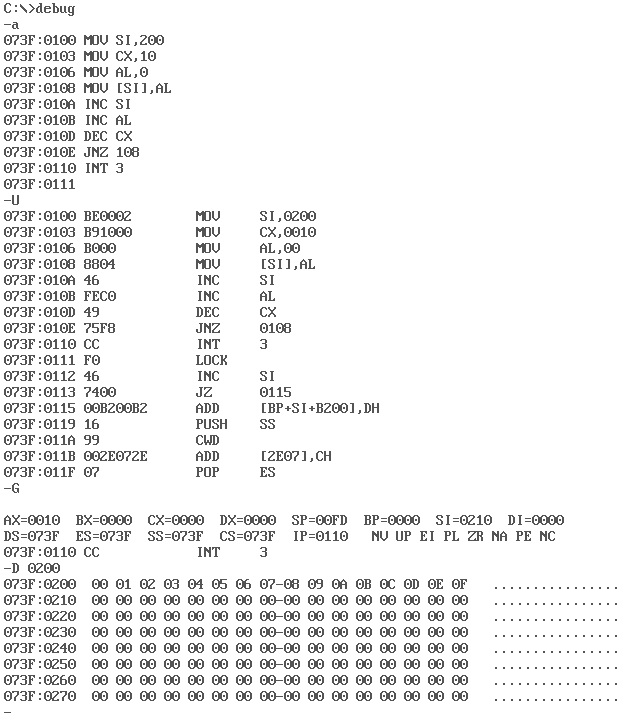
\includegraphics[width=\textwidth]{1-2.jpg}
\caption{1.1运行截图}
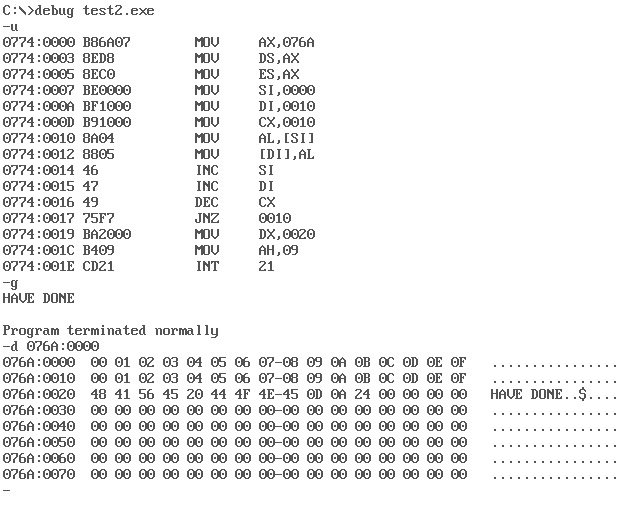
\includegraphics[width=\textwidth]{1-3.jpg}
\caption{1.2运行截图}
\end{figure}
\end{document}